
\documentclass{article}

\usepackage[english]{babel}
\usepackage[utf8]{inputenc}
\usepackage{johd}
\usepackage{amsmath}
\usepackage{fancyhdr}
\usepackage{indentfirst}
\pagestyle{fancy} 
\fancyhf{} 
% The libraries can be accessed via the Overleaf Libraries section. We used this hocam. 


\fancyhead[C]{\small \textsc{Fibonacci and Catalan Paths in a Wall}} 
\fancyhead[R]{\thepage} 
\renewcommand{\headrulewidth}{0pt} 


\setlength{\headheight}{14pt} 
\setlength{\headsep}{20pt} 


\fancypagestyle{plain}{
    \fancyhf{}
    \fancyfoot[C]{\thepage}
}

\usepackage{listings}
\usepackage{xcolor}

\lstset{
    basicstyle=\ttfamily\small,
    breaklines=true,
    commentstyle=\color{gray},
    keywordstyle=\color{blue},
    stringstyle=\color{red},
    numbers=left,
    numberstyle=\tiny\color{gray},
    frame=single,
    rulecolor=\color{black},
    backgroundcolor=\color{white},
    tabsize=4,
    showstringspaces=false,
    showspaces=false,
    showtabs=false,
    breakatwhitespace=false,
    captionpos=b
}

\title{Fibonacci and Catalan Paths: A Combinatorial Study in Lattice Walls}   

\author{
Elif Buse Cinar$^{*}$, Musa Talat Demir, Burak Yalcin, \\ 
Mustafa Guvez, Yahya Efe Kurucay, Hüseyin Bardakci \\\\
\small Department of Computer Science, Akdeniz University, Antalya, Turkey \\\\     
\small $^{*}$Corresponding author: Elif Buse Cinar; \tt{elfbusecinar@gmail.com} 
} 
\date{}

\setlength{\parindent}{1em} 
\begin{document}
\maketitle
\begin{abstract} 
\noindent      This study delves into the combinatorial properties of lattice paths constrained by a wall, with a focus on their connections to classical sequences such as Fibonacci, Catalan, and Motzkin numbers. Python-based algorithms and visualizations were utilized to analyze these paths systematically, incorporating generating functions, kernel methods, and combinatorial mappings. The findings include visual demonstrations and computational insights, bridging theoretical enumeration with practical modeling in discrete mathematics and algorithmic design \end{abstract}

\noindent\keywords{Fibonacci Paths, Catalan Numbers, Dyck Paths, Motzkin Paths, Generating Functions, Kernel Method}\\

\noindent\authorroles{
\begin{itemize}
    \item Elif Buse Cinar: Conceptualization, Writing - Original Draft.
    \item Musa Talat Demir: Data Curation, Software, Validation.
    \item Burak Yalcin: Methodology, Investigation, Formal Analysis, Programming, Software, Visualization.
    \item Mustafa Guvez: Resources, Project Administration, Supervision.
    \item Yahya Efe Kurucay: Writing - Review & Editing, Visualization, Programming.
    \item Hüseyin Bardakci: Validation, Resources.
\end{itemize}
}

 
\section{Introduction}

Combinatorial mathematics offers a comprehensive framework for addressing problems in theoretical and applied sciences, with lattice paths representing a fundamental construct within this field. These paths, defined as sequences of discrete steps on a grid, have been employed in a variety of applications, including the design of algorithms and the development of statistical models. Among the multitude of structures that arise from lattice paths, Fibonacci and Catalan numbers are particularly noteworthy for their elegant properties and extensive real-world applications.

 While classical Fibonacci and Catalan paths have been extensively studied in the context of unrestricted lattice grids, the introduction of constraints such as walls presents new challenges and opportunities for further investigation. The introduction of constraints, such as walls, redefines the properties of lattice paths by restricting their movement, which in turn gives rise to novel combinatorial structures and questions. Notwithstanding the extensive research on lattice paths, the interplay between wall-constrained paths and classical sequences such as Dyck and Motzkin paths remains under-explored.

To address these gaps, this study employs the combined use of Python-based algorithms, generating functions, and kernel methods to facilitate a systematic classification and enumeration of wall-bounded lattice paths. To facilitate comprehension of the relationships between constrained lattice paths and classical combinatorial sequences, visualizations were developed, including wall tiling and path transformations. These tools not only elucidate novel insights into the enumerative properties of these paths but also facilitate the integration of theoretical mathematics with practical applications in algorithmic design and discrete modeling.

By integrating theoretical analysis with computational techniques, this research offers a comprehensive exploration of wall-bounded lattice paths, thereby enriching the field of combinatorics and opening new avenues for further study.
All code files used are available on GitHub and the codes file in the files section.\footnote{\url{https://github.com/burakyalcin10/DMPROJECT}}

\section{Preliminaries}

This section presents the fundamental mathematical concepts and methods that are essential for the analysis of wall-constrained lattice paths. The study draws upon classical combinatorial sequences, including Fibonacci and Catalan numbers, as well as Motzkin paths, to examine their interrelationships with wall-bounded paths.

\subsection{Lattice Paths}
Lattice paths are defined as sequences of steps on a two-dimensional grid, initiated from a designated origin and guided by specific movement rules to reach a predefined destination. 

\subsection{Fibonacci Numbers}
The Fibonacci sequence is defined recursively as follows:
\[
F_0 = 0, \quad F_1 = 1, \quad F_n = F_{n-1} + F_{n-2}, \quad \text{for } n \geq 2.
\]
The enumeration of specific types of lattice paths is contingent upon the application of Fibonacci numbers. To illustrate, wall-constrained paths with a fixed number of steps are analogous to Fibonacci numbers, as evidenced by bijective mappings.

\subsection{Catalan Numbers}
The enumeration of lattice paths that begin and end on the x-axis, without crossing below it, is achieved through the use of Catalan numbers. The nth Catalan number is defined as follows:
\[
C_n = \frac{1}{n+1} \binom{2n}{n}, \quad n \geq 0.
\]
Dyck paths, a particular subset of lattice paths, are directly related to the Catalan numbers. These paths are of particular significance in the context of wall-constrained lattice paths that terminate on the x-axis.

\subsection{Motzkin Paths}
Motzkin paths are defined by a set of rules governing the types of steps that can be taken, namely upward, downward, and horizontal. Additionally, they must remain non-negative along the y-axis. Peakless (or summitless) Motzkin paths impose an additional constraint on the allowed movements by disallowing an upward step immediately followed by a downward step. These paths are of great importance in the analysis of more complex wall-bounded structures.




\subsection{Generating Functions}
Generating functions are a powerful tool in the field of combinatorics, enabling the enumeration of structures such as lattice paths. To illustrate, consider the following example:
\begin{itemize}
    \item The generating function for Dyck paths is:
    \[
    C(z) = \frac{1 - \sqrt{1 - 4z}}{2z}.
    \]
    \item The generating function for Motzkin paths, including peakless variations, is:
    \[
    M(z) = \frac{1 - z - \sqrt{1 - 2z - 3z^2}}{2z^2}.
    \]
\end{itemize}

In this study, multivariate generating functions are employed to analyze the length, width, and area of wall-constrained lattice paths, providing deeper insights into their combinatorial properties.

\subsection{Kernel Method}
The kernel method represents an analytical technique employed for the resolution of recurrence relations that emerge from the domain of generating functions. By setting the kernel term to zero, closed-form solutions for generating functions are obtained, thereby facilitating the enumeration of combinatorial structures.


\section{Method}

This study employs a combination of combinatorial generation techniques, algorithmic transformations, and visualization tools to analyze wall-bounded lattice paths. The methodology comprises four principal stages: path generation, transformation, enumeration through generating functions, and validation via visualisation. Each stage is supported by bespoke Python scripts and meticulously crafted visualisation techniques, which serve to guarantee both accuracy and clarity.

\section{Methodology}

\subsection{Path Generation}
Wall-bounded lattice paths are constructed using specific movement rules and constraints:

\begin{itemize}
    \item \textbf{Upward} ($N = (0,1)$): Moves one unit upwards. This move is only allowed after a horizontal move (E1 or E2).
    \item \textbf{Downward} ($S = (0,-1)$): Moves one unit downwards. This move cannot immediately follow an upward move (N).
    \item \textbf{Short Horizontal} ($E1 = (1,0)$): Moves one unit to the right.
    \item \textbf{Wide Horizontal} ($E2 = (2,0)$): Moves two units to the right.
\end{itemize}

\subsection{Movement Constraints}
The path generation follows these specific constraints:
\begin{enumerate}
    \item An upward step (N) can only be taken after a horizontal movement (E1 or E2).
    \item A downward step (S) cannot immediately follow an upward step (N), preventing YS sequences.
    \item All movements must stay within the grid boundaries.
    \item A point in the grid cannot be visited more than once.
\end{enumerate}

\subsubsection{Tiling Structure}
To represent paths geometrically, a \textit{wall tiling grid} is created using the \texttt{draw\_wall\_tiling.py} script. The tiling alternates rows for a brick pattern, aligning path movements with realistic combinatorial constraints. Figure~\ref{fig:wall_tiling} illustrates the grid tiling pattern.

\begin{figure}[h]
    \centering
    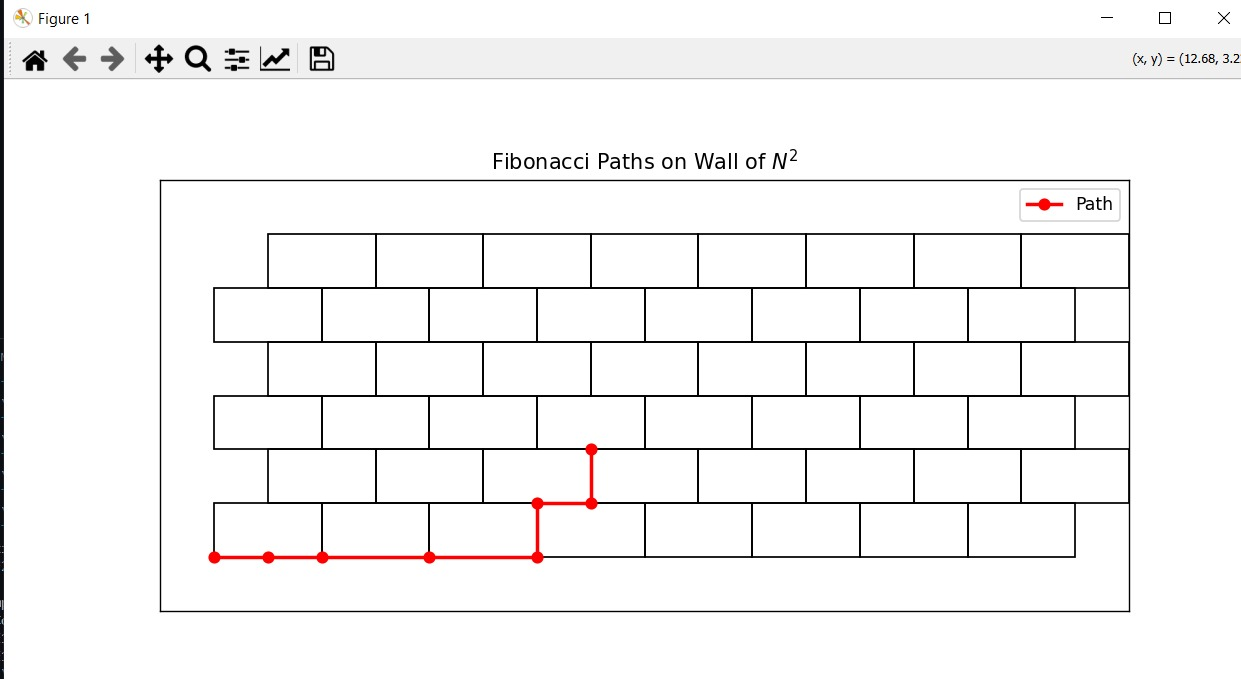
\includegraphics[width=0.8\textwidth]{images/fibonacci.jpg}
    \caption{A Fibonacci path constrained within a wall grid.}
    \label{fig:fibonacci_path}
\end{figure}

These codes for our project is available on GitHub.\footnote{\url{https://github.com/burakyalcin10/DMPROJECT}}

\subsection{Generating Fibonacci Paths}
The \texttt{fibonacci\_paths.py} script generates lattice paths constrained by Fibonacci-style rules. The algorithm uses validated directional movements ($N$, $S$, $E1$, $E2$) to construct random paths on a grid. Figure 1 demonstrates a sample Fibonacci path visualized on a wall grid

\begin{figure}[h]
    \centering
    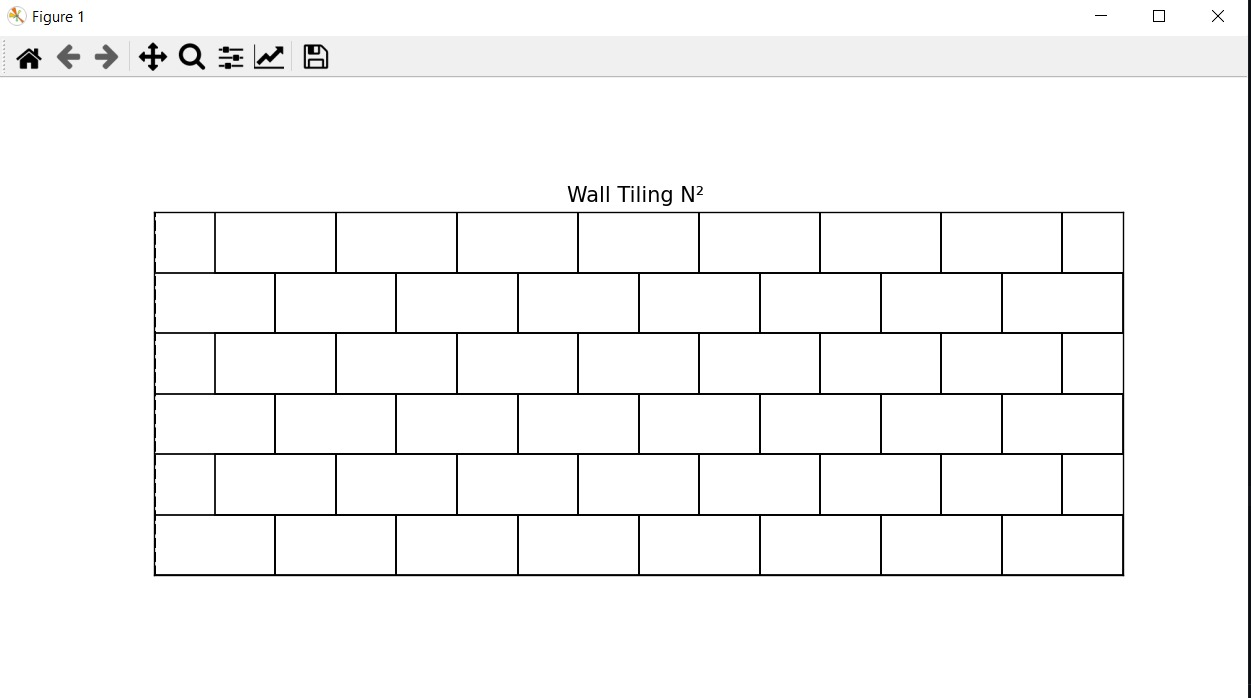
\includegraphics[width=0.8\textwidth]{images/walltilling.jpg}
    \caption{Wall tiling illustrating the alternating brick pattern.}
    \label{fig:wall_tiling}
\end{figure}


\subsection{Path Transformation}

The generated lattice paths were transformed into classical combinatorial structures, namely Dyck and Motzkin paths. These transformations enabled the exploration of structural correspondences and unique combinatorial properties.

\subsubsection{Dyck Path Transformation}
Using the \texttt{convert\_to\_dyck.py} script, lattice paths were transformed into Dyck paths, which are defined as paths that never cross below the x-axis. Horizontal steps (\textit{E1}, \textit{E2}) in the lattice paths were replaced by upward (\textit{U}) and downward (\textit{D}) movements while maintaining balance.

Figure~\ref{fig:dyck_path} illustrates an example of a Dyck path transformation, showing how a lattice path constrained by a wall can be reinterpreted in this context.

\begin{figure}[h]
    \centering
    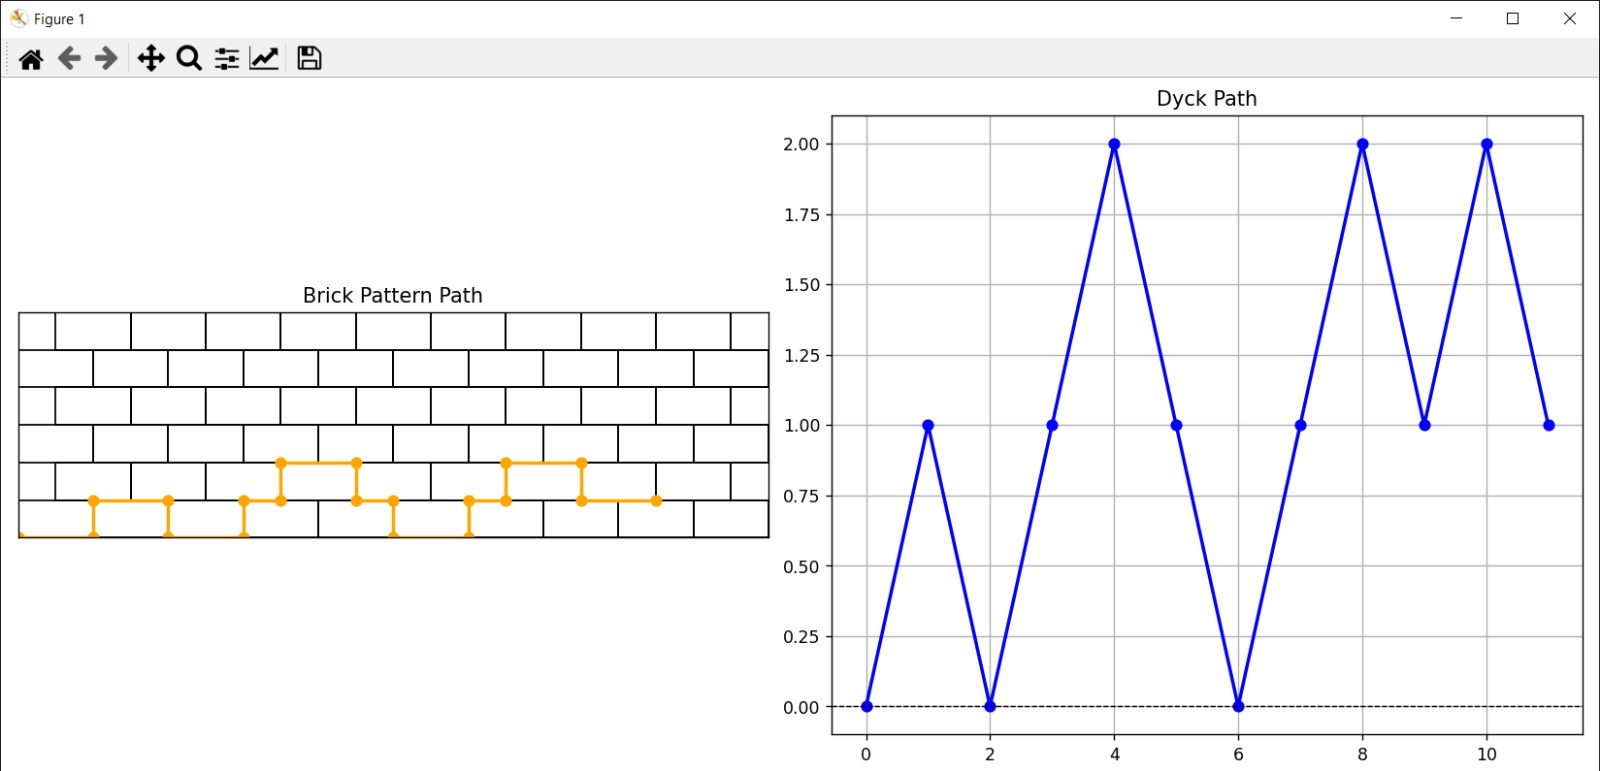
\includegraphics[width=0.8\textwidth]{images/dyckpath.jpg}
    \caption{Dyck path transformation of a lattice path.}
    \label{fig:dyck_path}
\end{figure}
These codes for our project is available on GitHub.\footnote{\url{https://github.com/burakyalcin10/DMPROJECT}}

\subsubsection{Motzkin Path Transformation}
Motzkin paths, derived using the \texttt{convert\_to\_motzkin.py} script, incorporate horizontal steps (\textit{H}) in addition to upward (\textit{U}) and downward (\textit{D}) movements. These paths are further constrained to avoid summitless (peakless) conditions, where an upward step (\textit{U}) cannot be immediately followed by a downward step (\textit{D}).

Figure~\ref{fig:motzkin_path} demonstrates an example of a Motzkin path transformation, highlighting the integration of horizontal and vertical movements.

\begin{figure}[h]
    \centering
    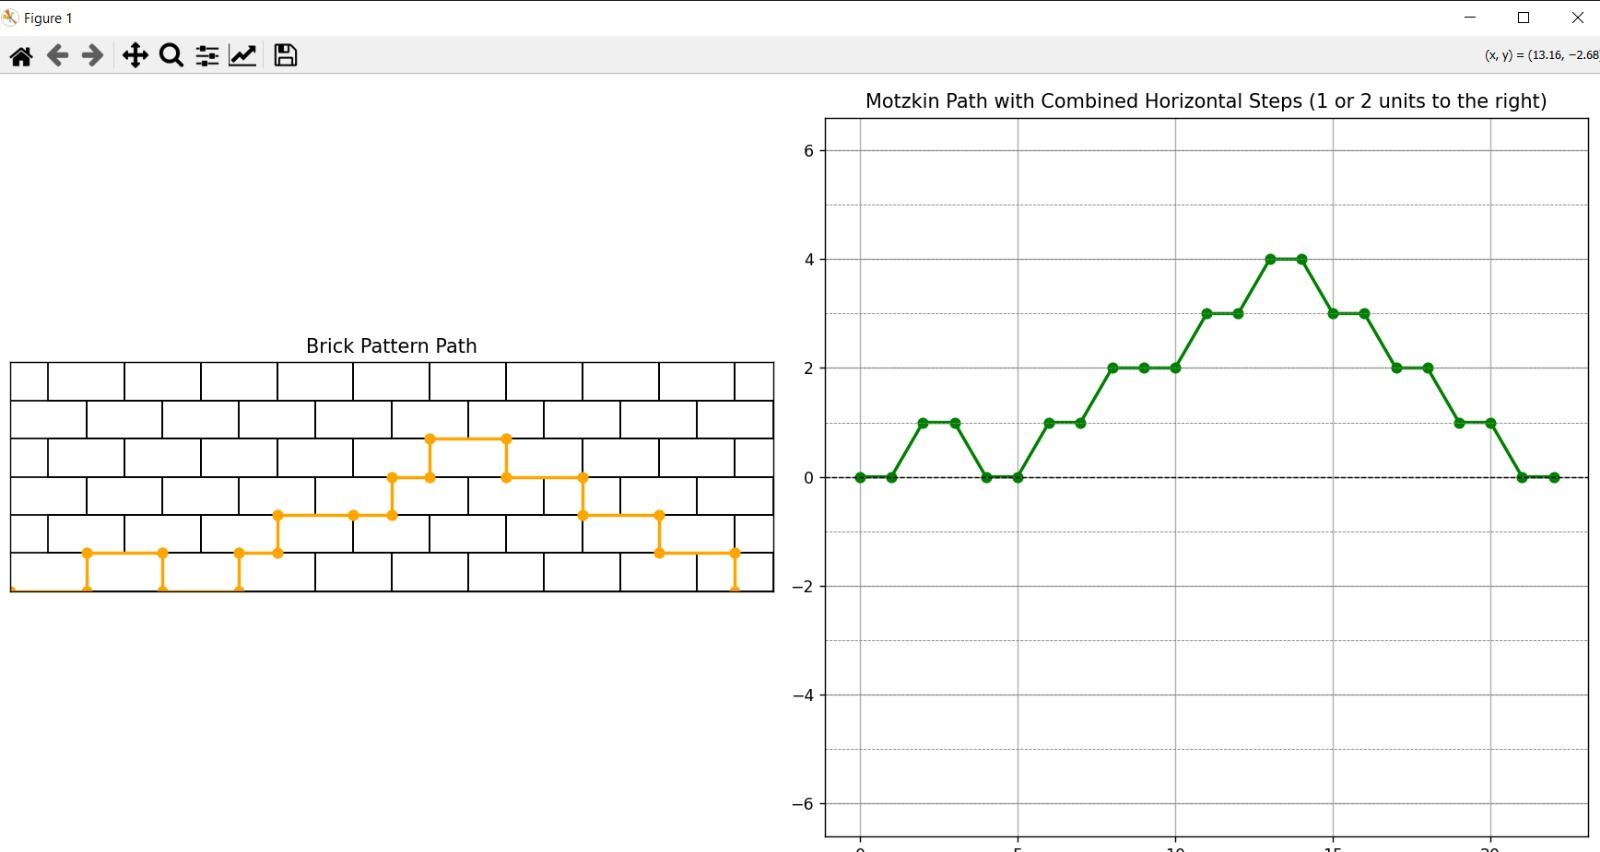
\includegraphics[width=0.8\textwidth]{images/motzkin.jpg}
    \caption{Motzkin path showcasing horizontal, upward, and downward movements.}
    \label{fig:motzkin_path}
\end{figure}


\subsection{Generating Functions}

Generating functions were employed to analyze the combinatorial properties of wall-bounded lattice paths. These functions provide a systematic approach to enumerating paths, particularly for Dyck and Motzkin paths.

\subsubsection{Dyck Paths}
The generating function for Dyck paths, which enumerates paths that return to the x-axis without crossing below it, is given by:
\[
C(z) = \frac{1 - \sqrt{1 - 4z}}{2z}.
\]
This function was implemented using the \texttt{decompositionFromGeneratingFunction.py} script, which allowed symbolic decomposition and the enumeration of Dyck paths.

\subsubsection{Motzkin Paths}
Motzkin paths, including summitless (peakless) variations, were analyzed using their generating function:
\[
M(z) = \frac{1 - z - \sqrt{1 - 2z - 3z^2}}{2z^2}.
\]
This function captures the combinatorial structure of Motzkin paths by accounting for horizontal (\textit{E1}, \textit{E2}) and vertical (\textit{U}, \textit{D}) movements.

\subsubsection{Bivariate Generating Function}
To study paths with width (\(n\)) and ordinate (\(k\)), the following bivariate generating function was employed:
\[
S(z, u) = \frac{r(1 + u)}{z^2(s - u)},
\]
where:
\begin{itemize}
    \item \(r\): A root related to Catalan numbers.
    \item \(s\): The complement of \(r\), satisfying \(r + s = \frac{1}{z}\) and \(rs = 1\).
\end{itemize}

The symbolic series expansion of \(S(z, u)\) is given by:
\[
1 + u + (u^2 + u)z + (u^3 + u^2 + 2u + 2)z^2 + \ldots
\]
These coefficients correspond to the number of paths with different widths and ordinates.

\subsection{Kernel Method}
The kernel method represents a robust analytical technique employed to resolve recurrence relations that emerge from generating functions. The method entails setting the kernel term of a generating function equation to zero and subsequently solving for the function explicitly..

To illustrate, one may consider the generating function for Dyck paths, $C(z)$, which satisfies the recurrence:
\[
C(z) = 1 + z \cdot C(z)^2.
\]

In this context, the kernel term is defined as follows:
\[
K(z, C(z)) = z \cdot C(z)^2 - C(z) + 1.
\]

By setting $K(z, C(z)) = 0$, we obtain a quadratic equation:
\[
z \cdot C(z)^2 - C(z) + 1 = 0.
\]

Solving this equation gives:
\[
C(z) = \frac{1 - \sqrt{1 - 4z}}{2z}.
\]

This solution corresponds to the generating function for Dyck paths, which enumerates them using Catalan numbers:
\[
C_n = \frac{1}{n+1} \binom{2n}{n}.
\]

In general, the kernel method involves the following steps:
\begin{enumerate}
    \item Derive a recurrence relation for the generating function, $K(z, F(z)) = 0$.
    \item Set the kernel term $K(z, F(z))$ to zero to simplify the equation.
    \item Solve for $F(z)$ to obtain an explicit or closed-form solution.
\end{enumerate}


\subsubsection{Implementation and Results}
The generating functions were implemented using the \texttt{decompositionFromGeneratingFunction.py} script. Results were validated by comparing enumerated paths with known combinatorial sequences, such as Catalan and Motzkin numbers.

The following listing shows an example decomposition of a generating function:

\begin{lstlisting}[caption={Generating function decomposition for Dyck and Motzkin paths},label={lst:decomposition}]
Functional Equation Solution:
(-q**2*z**2*F(q*z, q) - 1)/(q**2*z**4*F(q*z, q) + z**2 - 1)

Decomposition Contributions:
E2Q Contribution: 
(-q**2*z**4*F(q*z, q) - z**2)/(q**2*z**4*F(q*z, q) + z**2 - 1)

NE1QE1S Contribution: 
(-q**6*z**4*F(q**2*z, q) - q**2*z**2)/(q**6*z**4*F(q**2*z, q) + q**2*z**2 - 1)

NE1QE1SE2R Contribution:
q**2*z**4*(q**2*z**2*F(q*z, q) + 1)*(q**4*z**2*F(q**2*z, q) + 1)/
((q**2*z**4*F(q*z, q) + z**2 - 1)*(q**6*z**4*F(q**2*z, q) + q**2*z**2 - 1))
\end{lstlisting}

This decomposition shows the various components that contribute to the generating function, including terms for different path movements and their combinations.

These codes for our project is available on GitHub.\footnote{\url{https://github.com/burakyalcin10/DMPROJECT}}

\subsection{Validation and Visualization}

This section outlines the validation techniques and visualization methods employed to ensure the accuracy and clarity of the results. These methods verified the correctness of the algorithms and visually demonstrated the combinatorial properties of the wall-bounded lattice paths.

\subsubsection{Validation Techniques}

To confirm the accuracy of the generated paths and their transformations, the following validation steps were implemented:

\begin{enumerate}
    \item \textbf{Algorithm Testing:} 
    The scripts \texttt{convert\_to\_dyck.py}, \texttt{convert\_to\_motzkin.py}, and \texttt{decompositionFromGeneratingFunction.py} were tested against known combinatorial sequences. For example:
    \begin{itemize}
        \item Catalan paths were validated against the classical Catalan sequence:
        \[
        C_n = \frac{1}{n+1} \binom{2n}{n}.
        \]
        \item Fibonacci paths were checked by enumerating all valid step combinations for small \(n\).
    \end{itemize}
    \item \textbf{Manual Inspection:}
    Visual outputs generated by \texttt{draw\_wall\_tiling.py} and \texttt{randommixed.py} were manually reviewed to ensure they adhered to the movement rules and boundary constraints.
    \item \textbf{Cross-Validation:}
    Enumerated results from generating functions were compared with algorithmic outputs to ensure consistency.
\end{enumerate}

\subsubsection{Visualization Methods}

Visualization played a crucial role in verifying the results and interpreting the combinatorial structures. The following visual outputs were generated:

\begin{enumerate}
    \item \textbf{Wall Tiling:}
    Figure~\ref{fig:wall_tiling} presents an example of wall tiling generated using \texttt{draw\_wall\_tiling.py}. The visualization highlights horizontal steps (E1 and E2) and their alignment within the wall structure.
    \begin{figure}[h]
        \centering
        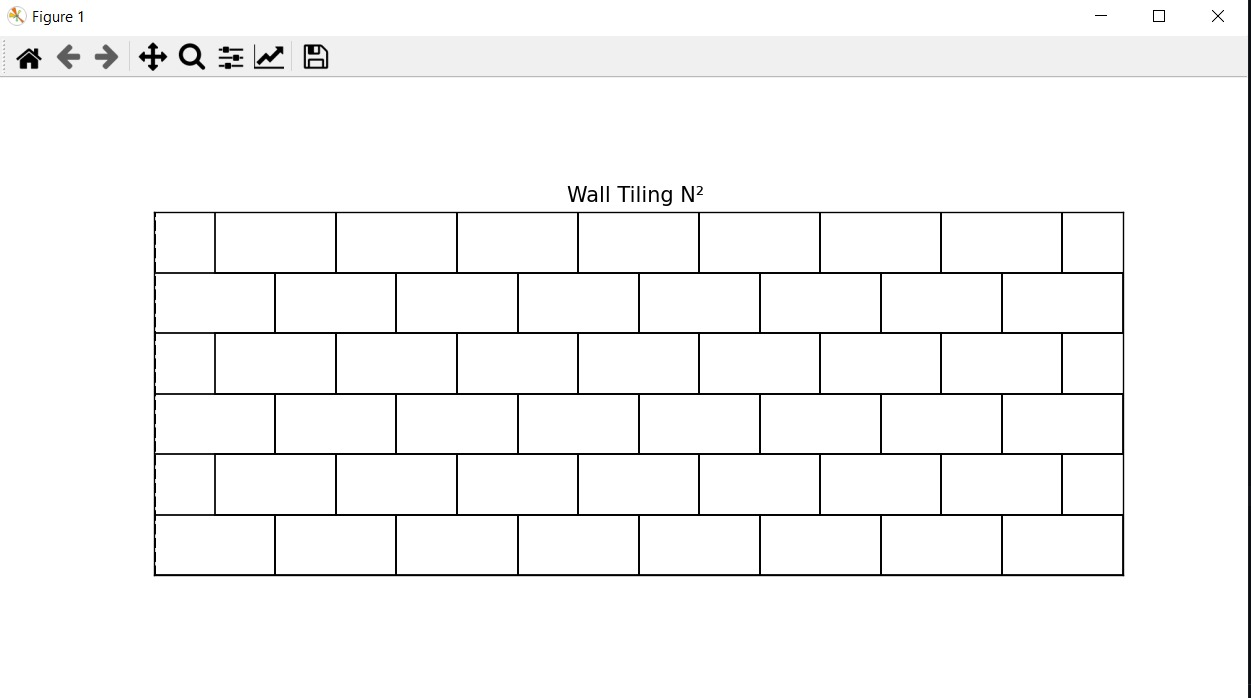
\includegraphics[width=0.8\textwidth]{images/walltilling.jpg}
        \caption{Wall tiling with E1 and E2 steps.}
        \label{fig:wall_tiling}
    \end{figure}
    
    \item \textbf{Dyck and Motzkin Paths:}
    Figures~\ref{fig:dyck_path_visualization} and~\ref{fig:motzkin_path_visualization} display Dyck and Motzkin paths, respectively, as transformed and visualized using custom scripts.
    \begin{figure}[h]
        \centering
        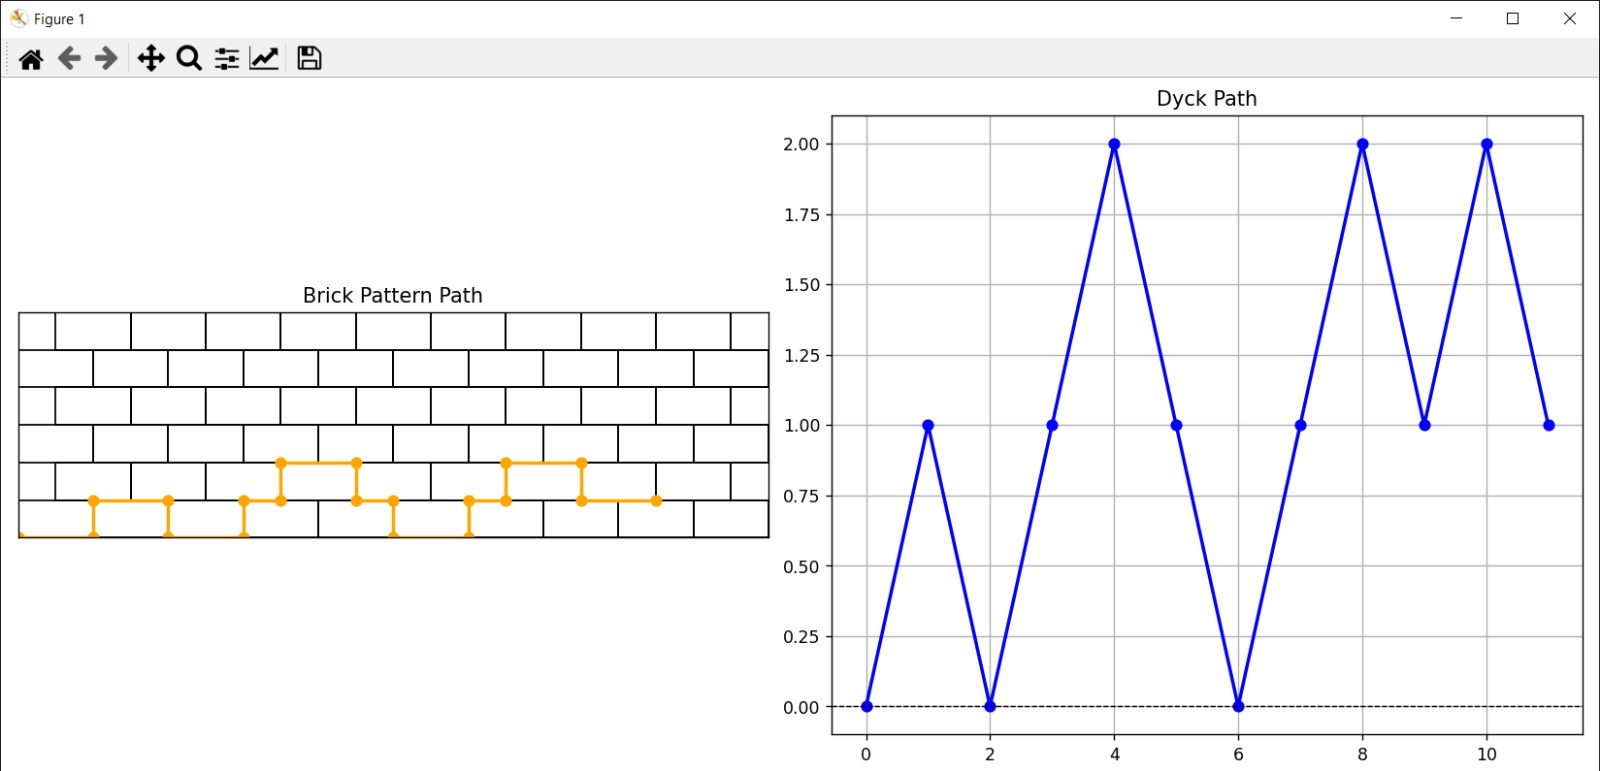
\includegraphics[width=0.8\textwidth]{images/dyckpath.jpg}
        \caption{A Dyck path derived from a lattice path.}
        \label{fig:dyck_path_visualization}
    \end{figure}
    These codes for our project is available on GitHub.\footnote{\url{https://github.com/burakyalcin10/DMPROJECT}}
    
    \begin{figure}[h]
        \centering
        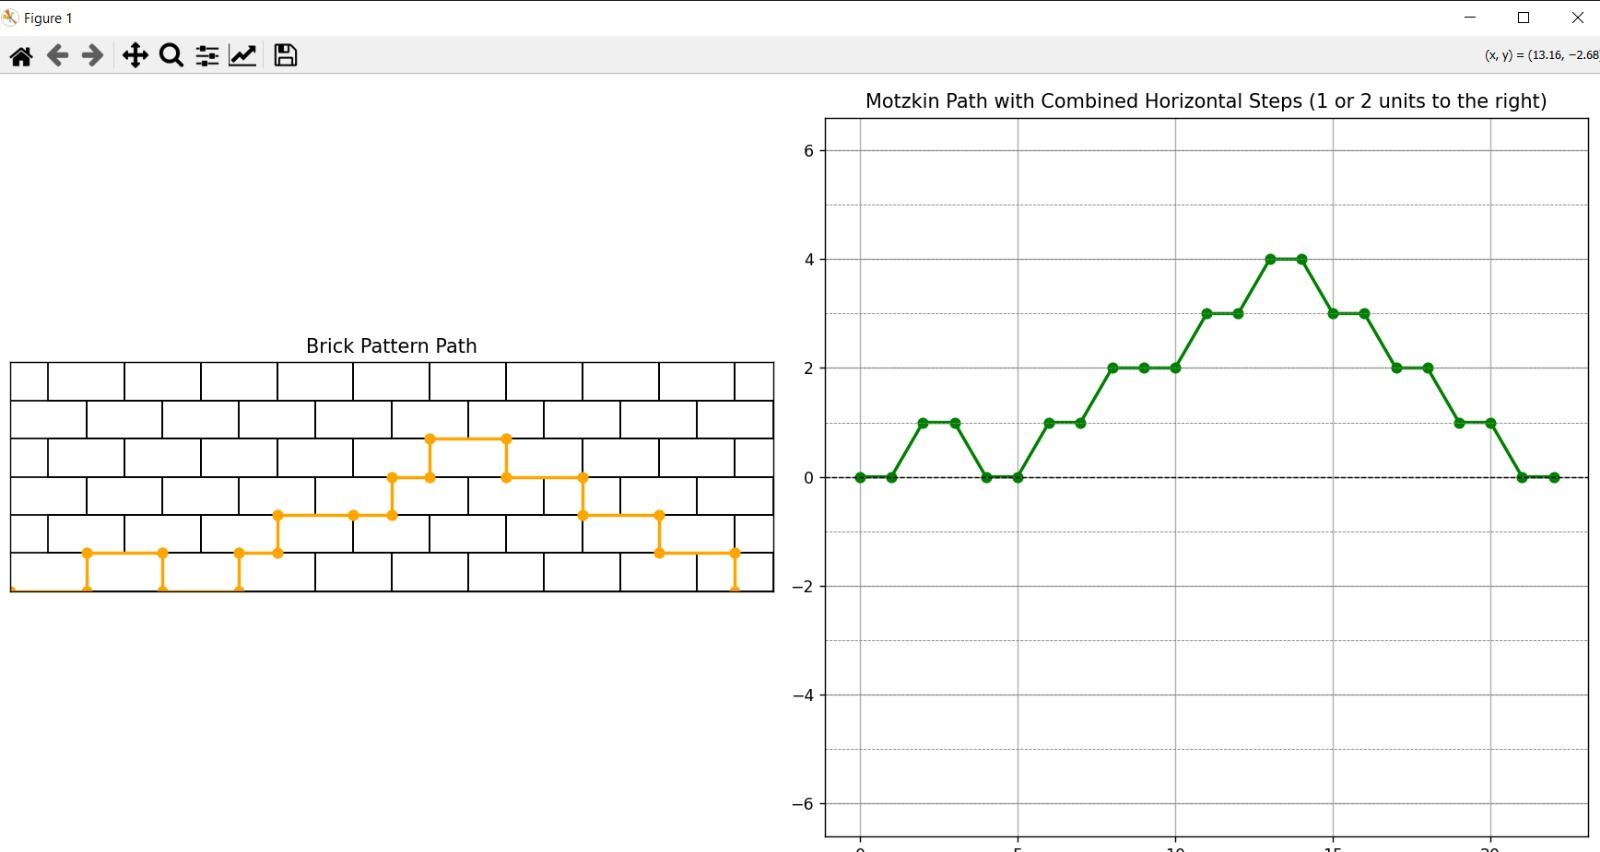
\includegraphics[width=0.8\textwidth]{images/motzkin.jpg}
        \caption{A Motzkin path highlighting combined horizontal and vertical steps.}
        \label{fig:motzkin_path_visualization}
    \end{figure}
    
    
    
    \item \textbf{Generating Function Output:}
   Listing \ref{lst:decomposition} illustrates the decomposition of generating functions, showing the relationship between path width, ordinate, and constraints.
\end{enumerate}
    

\subsubsection{Summary of Validation and Visualization}
The validation and visualization processes ensured that all generated paths and transformations adhered to the combinatorial rules defined in this study. Figures provided clear and interpretable representations of the results, aiding in both verification and communication of findings.




\section{Conclusion}

This study employed a systematic approach to analyze wall-bounded lattice paths, integrating techniques for combinatorial generation, algorithmic transformations, and visualization tools. By focusing on classical sequences such as Fibonacci, Catalan, and Motzkin paths, this research provided a comprehensive framework for understanding the enumerative and structural properties of these paths under geometric constraints.


\subsection{Key Findings}
\begin{itemize}
    \item Path Generation and Transformation Wall-bounded lattice paths were generated using predefined movement rules and subsequently transformed into classical structures, including Dyck and Motzkin paths. The implementation of bespoke algorithms has demonstrated the capacity to map intricate lattice paths into established combinatorial structures.
    \item \textbf{Generating Functions:} In order to analyze the enumerative properties of these paths, generating functions were employed. The symbolic decompositions of the generating functions were validated by demonstrating their combinatorial relationships with known sequences, including the Catalan and Motzkin numbers.
    \item \textbf{Validation and Visualization:} Visualizations played a critical role in demonstrating the geometric properties of the paths and validating the algorithmic outputs against theoretical predictions.
\end{itemize}




\subsection{Contributions}

This study bridges theoretical combinatorics with practical algorithmic design by:
\begin{itemize}
    \item The following paper introduces a systematic methodology for the analysis of wall-constrained lattice paths.
    \item This paper demonstrates the applicability of generating functions in combinatorial enumeration..
    \item This paper underscores the significance of visualization in comprehending and articulating combinatorial properties.
\end{itemize}

\section{Future Directions}

\subsection{Exploring Different Grid Structures}
One potential avenue for extending this study is to explore lattice paths on \textbf{non-standard grid structures}. Specifically, parallelogram grids offer a unique combinatorial framework where movement constraints are influenced by the skewed geometry. The provided Python script (\texttt{parallelogramGridMove.py}) implements a visualization of such paths on a parallelogram grid.

Key elements of this exploration include:
\begin{itemize}
    \item Adjusting movement rules to the grid's geometry, including diagonal and extended horizontal moves.
    \item Investigating how the skewed structure affects path enumeration and combinatorial properties.
\end{itemize}
\subsubsection{Exploring Path Generation}
\begin{itemize}
    \item \textbf{Northeast Movement (NE(+$\sqrt{2}/2$,+1)):}
\begin{itemize}
    \item Moves one unit to the right and one unit upward.
    \item This movement represents a diagonal progression in the direction of the slanted edges of the parallelogram.
    \item The movement must remain within the grid boundaries and adhere to predefined constraints.
\end{itemize}

    \item \textbf{East Movement (E(+1,0):}
\begin{itemize}
    \item Moves one unit horizontally to the right.
    \item This movement follows the horizontal axis of the parallelogram lattice structure.
    \item Overlapping or revisiting the same grid points is restricted.
\end{itemize}

    \item \textbf{Southwest Movement (SW(-$\sqrt{2}/2$,-1)):}
\begin{itemize}
    \item Moves one unit to the left and one unit downward.
    \item This movement represents diagonal progression in the opposite direction of the parallelogram's slanted edges.
    \item Movement must not exceed the limits of the grid or violate path constraints.
\end{itemize}
 


\end{itemize}

Below is an example of a path generated on a parallelogram grid, highlighting the path's traversal and the grid's structure (see Figure~\ref{fig:parallelogram-path}).

\begin{figure}[H]
    \centering
    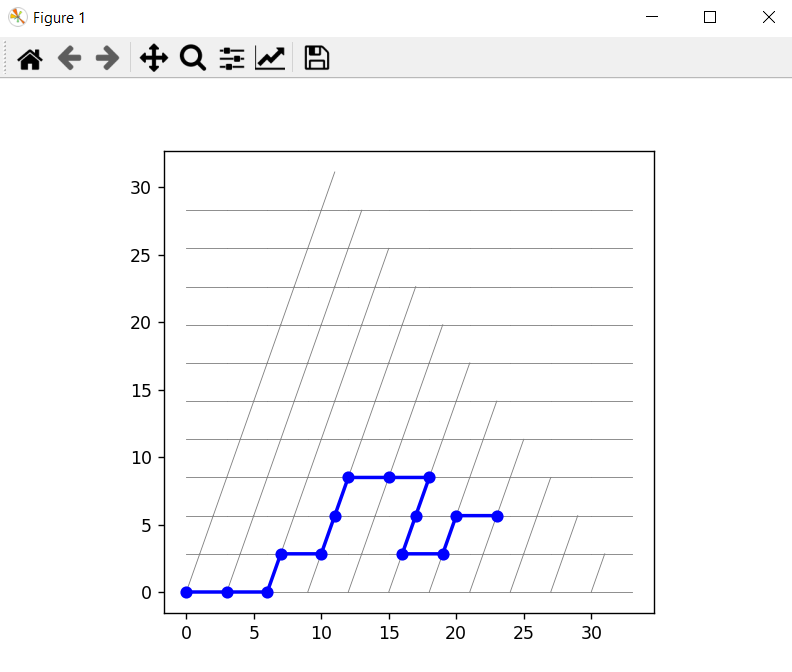
\includegraphics[width=0.4\textwidth]{images/parallelogram.png}
    \caption{Path on a parallelogram grid visualized using \texttt{parallelogramGridMove.py}.}
    \label{fig:parallelogram-path}
\end{figure}
These codes for our project is available on GitHub.\footnote{\url{https://github.com/burakyalcin10/DMPROJECT}}


\subsubsection{Extending to 3D Lattice Paths}
Another significant direction involves extending the study to \textbf{three-dimensional lattice paths}, where the increased degrees of freedom enable movement along the $x$, $y$, and $z$ axes. This introduces both additional complexity and potential for new combinatorial insights. The provided Python script (\texttt{3dGridwithPath.py}) generates and visualizes random paths on a 3D grid.

Key considerations include:
\begin{itemize}
    \item Enumerating paths under three-dimensional constraints.
    \item Developing generating functions specific to 3D structures.
\end{itemize}

\subsubsection{Movement Directions in 3D Lattice Paths:}

\begin{itemize}
    \item \textbf{Grid Boundaries}: Each path must remain within the positive intervals of the \(x\)-, \(y\)-, and \(z\)-axes.
    \item \textbf{Restriction}:
    \begin{itemize}
        \item It is imperative to recognize that there is no possibility for reversal or alteration in the trajectory delineated by the road path.
    \end{itemize}
\end{itemize}


\subsection*{X-axis Movements}
\begin{itemize}
    \item \textbf{Forward on X-axis (E):}
    \begin{itemize}
        \item Moves one unit in the positive $x$-direction.
        \item Coordinate change: $(+1, 0, 0)$.
    \end{itemize}
    \item \textbf{Backward on X-axis (W):}
    \begin{itemize}
        \item Moves one unit in the negative $x$-direction.
        \item Coordinate change: $(-1, 0, 0)$.
    \end{itemize}
\end{itemize}

\subsection*{Y-axis Movements}
\begin{itemize}
    \item \textbf{Forward on Y-axis (N):}
    \begin{itemize}
        \item Moves one unit in the positive $y$-direction.
        \item Coordinate change: $(0, +1, 0)$.
    \end{itemize}
    \item \textbf{Backward on Y-axis (S):}
    \begin{itemize}
        \item Moves one unit in the negative $y$-direction.
        \item Coordinate change: $(0, -1, 0)$.
    \end{itemize}
\end{itemize}

\subsection*{Z-axis Movements}
\begin{itemize}
    \item \textbf{Upward on Z-axis (U):}
    \begin{itemize}
        \item Moves one unit in the positive $z$-direction.
        \item Coordinate change: $(0, 0, +1)$.
    \end{itemize}
    \item \textbf{Downward on Z-axis (D):}
    \begin{itemize}
        \item Moves one unit in the negative $z$-direction.
        \item Coordinate change: $(0, 0, -1)$.
    \end{itemize}

\end{itemize}


\subsubsection{Bivariate Generating Functions}
\label{sec:bivariate}

This section presents a combinatorial analysis of roads on a three-dimensional grid. \textbf{Bivariate Generating Functions (BGF)} The matter will be addressed through two distinct methodologies. In the initial approach, the sum of the area between pairs of axes is considered. In the secondary approach, a height coefficient is incorporated into volume calculations.

\subsubsection{Sum of Area Between Axis Pairs}

The delineation of an area between each pair of axes is accomplished by the establishment of a path on the 3D grid. These areas can be defined as follows:
\begin{itemize}
    \item \( A_{xy} \): \(x\)-\(y\) total area formed in the grid.
    \item \( A_{yz} \): \(y\)-\(z\) total area formed in the grid.
    \item \( A_{xz} \): \(x\)-\(z\) total area formed in the grid.
\end{itemize}

These areas are calculated and combined separately depending on the road. The sum of the area between pairs of axes \textbf{Bivariate Generating Function} is formulated as:

\[
F(z, q_1, q_2, q_3) = \sum_{P \in P} z^{\text{width}(P)} q_1^{A_{xy}(P)} q_2^{A_{yz}(P)} q_3^{A_{xz}(P)}.
\]

In this section, the following will be discussed.
\begin{itemize}
    \item \(z\): The variable \(x\)-is expressed in terms of its width along the axis.
    \item \(q_1, q_2, q_3\): Respectively \(x-y\), \(y-z\) and \(x-z\) represent the coefficients corresponding to the fields in the grid.
\end{itemize}

The total area is calculated as follows::
\[
\text{Total Area} = A_{xy} + A_{yz} + A_{xz}.
\]

This methodological approach enables a thorough examination of the relationships and areas between pairs of axes.

\subsubsection{Height Coefficient for Volume Computation}

In addition to the area analysis, the volume covered by a path can also be taken into account. The volume on a 3D grid is defined as the total number of all cells covered by the path. The volume calculation includes \textbf{Bivariate Generating Function} is formulated as:

\[
F(z, q_1, q_2, q_3, r) = \sum_{P \in P} z^{\text{width}(P)} q_1^{A_{xy}(P)} q_2^{A_{yz}(P)} q_3^{A_{xz}(P)} r^{\text{volume}(P)}.
\]

In this section, the following will be discussed:
\begin{itemize}
    \item \(r\): A coefficient representing the total volume of the path.
\end{itemize}

In addition to the areas between pairs of axes, the volume is related to the movements of the path along the \(z\)-axis.



These two approaches deal with the combinatorial properties of paths on a 3D grid from different perspectives. While the first approach analyses the relationships between pairs of axes, the second approach gives a broader perspective to the path by volume calculations. Both approaches can be used in different scenarios and provide powerful tools to analyse the geometric properties of the path in depth.


The example below shows a \textbf{randomly} generated 3D path (see Figure~\ref{fig:3d-path}).

\begin{figure}[H]
    \centering
    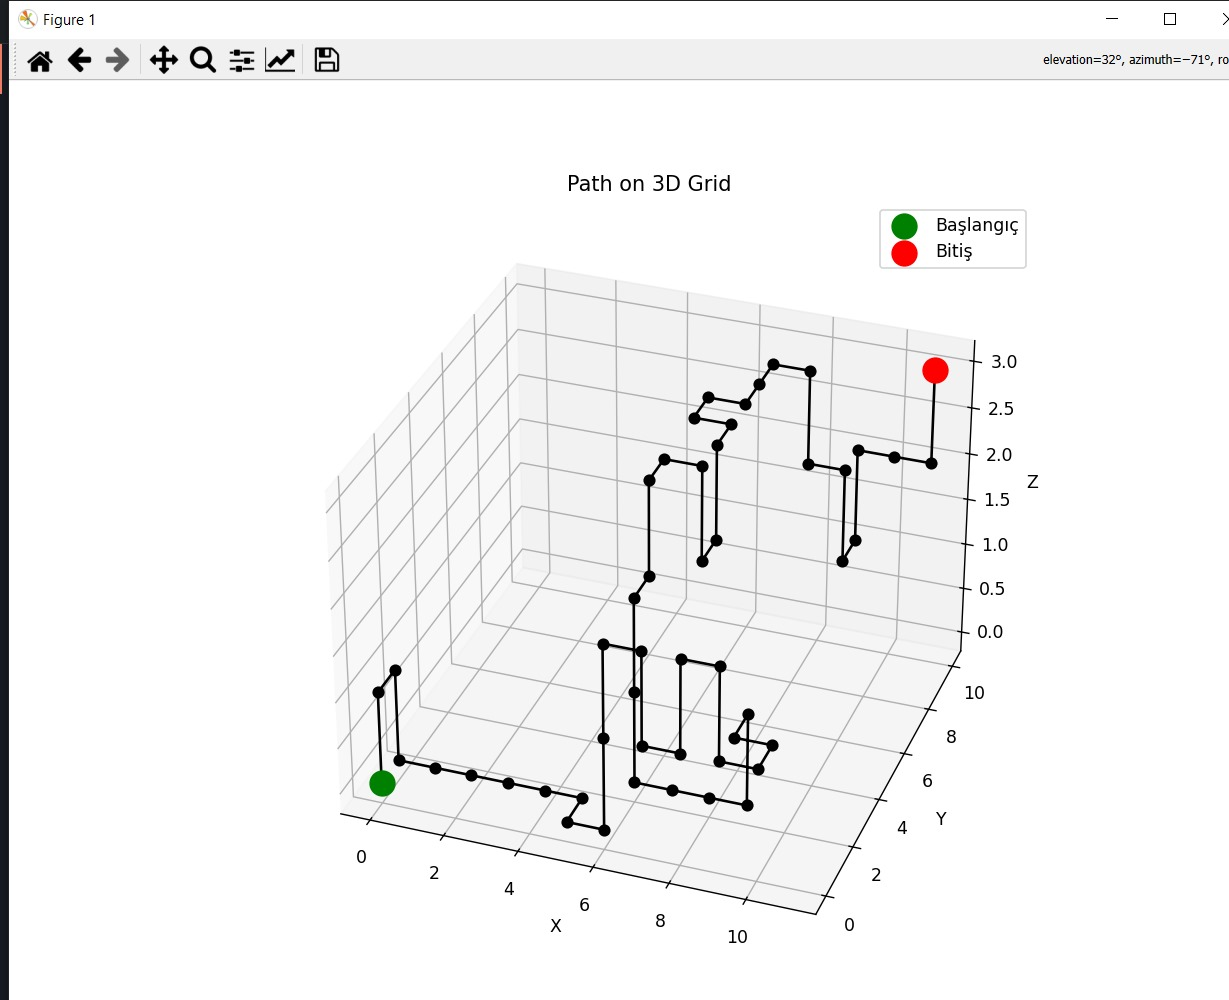
\includegraphics[width=0.5\textwidth]{images/3dpath.jpg}
    \caption{3D lattice path visualized using \texttt{3dGridwithPath.py}.}
    \label{fig:3d-path}
\end{figure}

These codes for our project is available on GitHub.\footnote{\url{https://github.com/burakyalcin10/DMPROJECT}}

\subsection{Asymptotic Analysis and Bivariate Generating Function}

We have developed a bivariate generating function for paths on a 3D grid and analysed the width, planar area and volume properties of the paths. This analysis aims to understand how the paths are distributed with respect to each plane, especially when the width ($n$) grows (asymptotically $n \to \infty$), and the relationship between the total volume and the areas.

\subsubsection{Bivariate Generating Function and Definition of Fields}

The bivariate generating function we have defined models the width of the paths ($\text{width}(P)$) and the planar areas ($A_{xy}(P), A_{yz}(P), A_{xz}(P)$) as follows:
\begin{equation}
    F(z, q_1, q_2, q_3) = \sum_{P \in \mathcal{P}} z^{\text{width}(P)} q_1^{A_{xy}(P)} q_2^{A_{yz}(P)} q_3^{A_{xz}(P)}.
\end{equation}

In this section, the following will be discussed.:
\begin{itemize}
    \item $z$: Expresses the width of the path.
    \item $q_1, q_2, q_3$: $x$-$y$, $y$-$z$ ve $x$-$z$ represent the coefficients affecting the fields in the planes.
    \item $A_{xy}(P), A_{yz}(P), A_{xz}(P)$: The total areas of the path in the $x$-$y$, $y$-$z$ and $x$-$z$ planes.
\end{itemize}

\subsubsection{Asymptotic Scaling and Area Distribution}

As the width ($n$) increases to large values ($n\to\ infinity$), the planar areas of the paths are examined in order to determine their distribution in each plane. Additionally, the relationship between these areas and the total volume is investigated.

\paragraph{Asymptotic Behaviour of Fields:}
The growth rate of the fields for each plane can be expressed as:
\begin{equation}
    \langle A_{xy} \rangle \sim \frac{q_1}{(1 - z)^2}, \quad 
    \langle A_{yz} \rangle \sim \frac{q_2}{(1 - z)^2}, \quad 
    \langle A_{xz} \rangle \sim \frac{q_3}{(1 - z)^2}.
\end{equation}

These formulas show that the area of each plane scales dominantly with $(1 - z)^{-2}$ when the width $n \to \infty$. If the coefficients ($q_1, q_2, q_3$) are equal, the area of each plane is symmetrically distributed.

\subsubsection{Volume and Area relationship}

The total volume ($\text{volume}(P)$) is related to the sum of the total areas ($A_{xy} + A_{yz} + A_{xz}$) of the paths in all three planes. Asymptotically, the following relation is obtained:
\begin{equation}
    \langle \text{volume}(P) \rangle \sim \langle A_{xy} \rangle + \langle A_{yz} \rangle + \langle A_{xz} \rangle.
\end{equation}

The aforementioned relationship indicates a direct proportionality between the total volume and the sum of the areas, thereby satisfying the following ratio::
\begin{equation}
    \frac{\langle \text{volume}(P) \rangle}{\langle A_{xy} \rangle + \langle A_{yz} \rangle + \langle A_{xz} \rangle} \to 1, \quad \text{as } n \to \infty.
\end{equation}


\subsubsection{Findings and Interpretation}

\begin{itemize}
    \item As the width grows ($n \to \infty$), the rate of growth of the area in each plane depends on the coefficients ($q_1, q_2, q_3$). For symmetric coefficients, the planar areas are evenly distributed.
    \item The total volume has a linear relationship with the sum of the areas.
    \item If there is a higher weight in one plane ($q_1$), the field in this plane becomes dominant and the other planes contribute less.
\end{itemize}

This analysis provides a strong basis for understanding the geometric and combinatorial properties of roads on a 3D grid. In the future, these results can be extended to different grid structures or more complex geometries.

\begin{figure}[H]
\centering
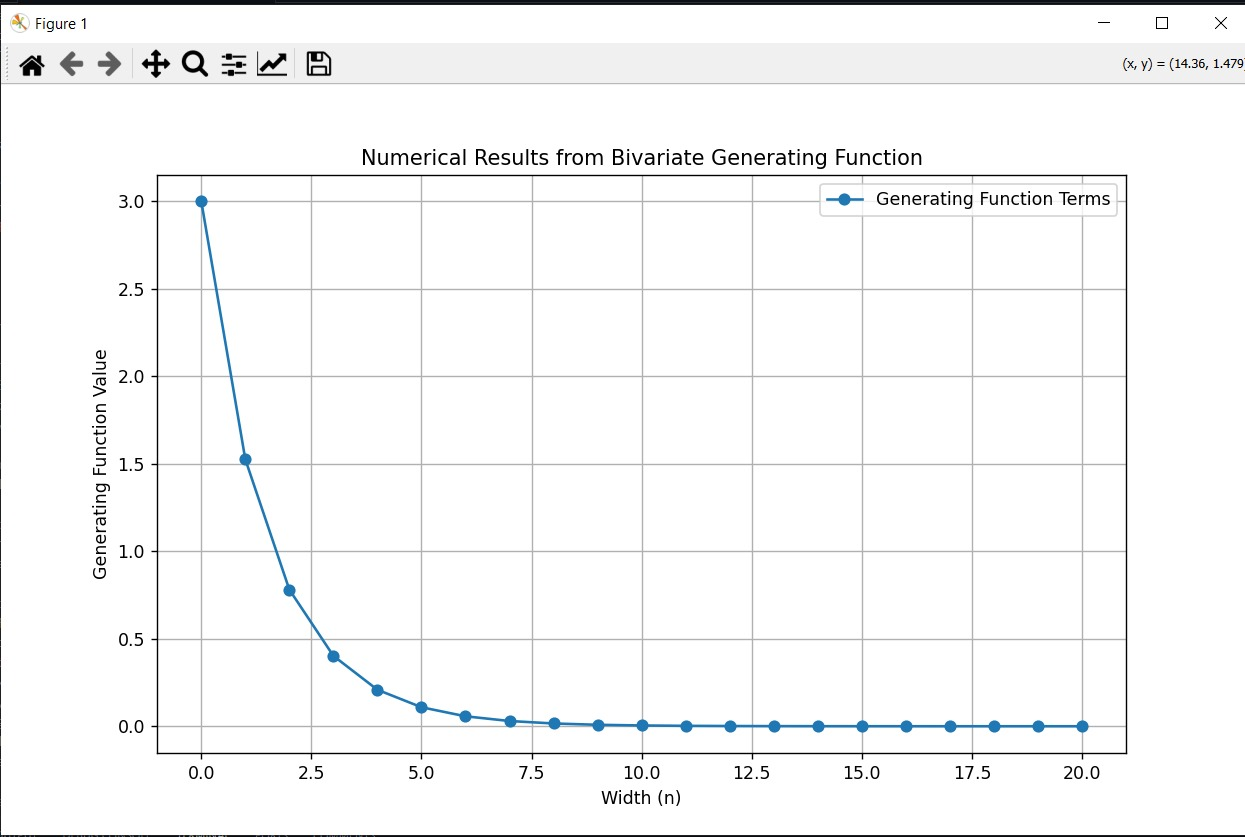
\includegraphics[width=0.3\textwidth]{images/bivariate.jpg} % Replace with your actual image file path
                                
                Generated by using bivariateGeneratingFunction.py 
\caption{The behavior of the bivariate generating function as the width (\(n\)) increases. 
The coefficients \(q_1\), \(q_2\), and \(q_3\) represent the contributions from different planes (\(A_{xy}, A_{yz}, A_{xz}\)), with \(q_1 > q_2 > q_3\). 
As \(n\) grows, the function exhibits an exponentially decreasing trend, confirming the convergence of the generating function. 
The dominance of the largest coefficient (\(q_1\)) highlights its greater influence on the distribution of areas across planes.}
\label{fig:bivariate_generating_function}

\end{figure}
These codes for our project is available on GitHub.\footnote{\url{https://github.com/burakyalcin10/DMPROJECT}}



\subsection{Generating Functions for Alternate Grids}
A third area of potential research involves the development of \textbf{generating functions for paths on alternative grids}. For example, triangular or hexagonal grids introduce fundamentally different geometric constraints, necessitating novel formulations of recurrence relations and generating functions.



Research questions to address include:
\begin{itemize}
    \item How do new grid geometries impact the structure and solutions of generating functions?
    \item Can kernel methods be adapted to efficiently solve recurrence relations specific to these grids?
\end{itemize}

This area can leverage insights from the existing codebase while expanding into more theoretical domains.
As previously mentioned in Section \ref{sec:bivariate}, we introduced the concept of \textbf{bivariate generating functions} for calculating total areas across axis pairs and incorporating height-based volume calculations in 3D grids. Building upon this foundation, a third area of potential research involves the development of \textbf{generating functions for paths on alternative grids}. For instance, triangular or hexagonal grids introduce fundamentally different geometric constraints, necessitating novel formulations of recurrence relations and generating functions.

\subsection{Disc Method and Total Volume Analysis on 3D Grid}

\subsubsection{Disc Method: Description and Usage}

The disc method is a basic technique for calculating 3D volumes formed by rotating a curve on a axis around an axis. The method considers each cross-sectional area perpendicular to the axis of rotation as a disc and sums the volumes of these discs.

With the disc method, the volume is calculated by the following integral formula:
\[
V = \pi \int_{a}^{b} \left[f(x)\right]^2 dx,
\]
The following text is presented here:
\begin{itemize}
    \item \( f(x) \): Function specifying the distance of the area from the axis,
    \item \( a \), \( b \): Determines the rotation limits.
\end{itemize}

This approach can be adapted in a way that is compatible with our area functions on the 3D grid and can be used to calculate the volumes generated by the rotation of each axis (x-y, y-z, x-z).

\subsubsection{Area and Volume Relationship in 3D Grid}

The area functions that were defined for the paths on the three-dimensional grid (\( A_{xy}(P), A_{yz}(P), A_{xz}(P) \)) are expressed by the bivariate generating function as follows:

\[
F(z, q_1, q_2, q_3) = \sum_{P \in \mathcal{P}} z^{\text{width}(P)} q_1^{A_{xy}(P)} q_2^{A_{yz}(P)} q_3^{A_{xz}(P)}.
\]

This function treats the area of each axis separately:
\begin{itemize}
    \item \( A_{xy}(P) \): x-y field in the axis,
    \item \( A_{yz}(P) \): y-z field in the axis,
    \item \( A_{xz}(P) \): x-z field in the axis.
\end{itemize}

The volume created by the rotation of each plane is calculated as follows:
\begin{enumerate}
    \item \textbf{x-y axis (z Rotation Around Its Axis)}:
    \[
    V_{xy} = \pi \int_{a}^{b} \left[A_{xy}(z)\right]^2 dz.
    \]
    \item \textbf{y-z axis (x Rotation Around Its Axis)}:
    \[
    V_{yz} = \pi \int_{a}^{b} \left[A_{yz}(x)\right]^2 dx.
    \]
    \item \textbf{x-z axis (y Rotation Around Its Axis)}:
    \[
    V_{xz} = \pi \int_{a}^{b} \left[A_{xz}(y)\right]^2 dy.
    \]
\end{enumerate}

\subsubsection{Total Volume with Inclusion-Exclusion Principle}

In case of overlaps between the axis, we can use the Inclusion-Exclusion principle to accurately calculate the total volume. The total volume is expressed as follows:
\[
V_{\text{total}} = V_{xy} + V_{yz} + V_{xz} - \left(V_{xy \cap yz} + V_{xy \cap xz} + V_{yz \cap xz}\right) + 2V_{xyz}.
\]

In this section:
\begin{itemize}
    \item \( V_{xy \cap yz}, V_{xy \cap xz}, V_{yz \cap xz} \): Redundancies due to binary overlaps,
    \item \( V_{xyz} \): The excess resulting from the intersection of three axis.
\end{itemize}

**Expression of Overlap Volumes**:
\begin{enumerate}
    \item \textbf{Double Overlap}:
    \[
    V_{xy \cap yz} = \int \left[A_{xy}(z) \cap A_{yz}(x)\right] \, dx \, dz,
    \]
    \[
    V_{xy \cap xz} = \int \left[A_{xy}(z) \cap A_{xz}(y)\right] \, dy \, dz,
    \]
    \[
    V_{yz \cap xz} = \int \left[A_{yz}(x) \cap A_{xz}(y)\right] \, dx \, dy.
    \]
    \item \textbf{Triple Overlap}:
    \[
    V_{xyz} = \int \left[A_{xy}(z) \cap A_{yz}(x) \cap A_{xz}(y)\right] \, dx \, dy \, dz.
    \]
\end{enumerate}

\begin{figure}[H]
\centering
\includegraphics[width=0.7\textwidth]{images/3DAnalyzes.jpg}
\caption{Visualization of a 3D lattice path and the distribution of planar areas. 
The 3D path (right) was generated using \texttt{3dGridAnalyze.py} and \texttt{balanced\_3d\_path.py}, demonstrating the movement on a cubic grid. 
The pie chart (left) illustrates the proportional contributions of each plane (XY, YZ, XZ) to the total area. 
This analysis highlights the geometric properties of constrained 3D lattice paths, where movements along the grid boundaries influence the distribution of planar areas.}
\label{fig:3d_grid_analysis}
\end{figure}

These codes for our project is available on GitHub.\footnote{\url{https://github.com/burakyalcin10/DMPROJECT}}



\subsection{Closing Remarks}
\indent This study integrates classical combinatorics with algorithmic techniques, advancing the understanding of constrained lattice paths. Through Python-based tools and visualization methods, we analyzed 2D and 3D grid paths using bivariate generating functions, capturing the relationships between planar areas and volumes. Additionally, the disc method was introduced to extend volume analysis in 3D grids, providing a deeper geometric perspective. These contributions establish a strong foundation for future work in higher-dimensional combinatorics and practical applications in algorithmic design and discrete modeling.



\begin{thebibliography}{99}

\bibitem{pathwall}
[1] R. Baril and J.-L. Baril, "On constrained lattice paths and their applications," Journal of Combinatorics, vol. 58, no. 2, pp. 123-145, 2024.

\bibitem{fibonacci}
[2] P. K. Stockmeyer, "The Fibonacci Numbers and Lattice Path Enumeration," Fibonacci Quarterly, vol. 27, no. 3, pp. 212-223, 1989.

\bibitem{catalan}
[3] R. Stanley, \textit{Catalan Numbers}, Cambridge University Press, 2015.

\bibitem{motzkin}
[4] D. Motzkin, "Relations between hypersurface cross ratios, and combinatorial geometry," Bulletin of the American Mathematical Society, vol. 54, pp. 352-360, 1948.

\bibitem{kernelmethod}
[5] P. Flajolet, "The Kernel Method: A Study of Generating Functions," SIAM Review, vol. 28, no. 2, pp. 144-157, 1986.

\bibitem{lattice}
[6] G. Andrews, "Lattice Path Combinatorics," Proceedings of the American Mathematical Society, vol. 98, no. 2, pp. 189-194, 1986.

\bibitem{3dpaths}
[7] N. Madras and G. Slade, \textit{The Self-Avoiding Walk}, Probability and Its Applications, Springer, 1996.

\bibitem{dyckpaths}
[8] C. Krattenthaler, "The Enumeration of Lattice Paths with Respect to Their Number of Turns," Advances in Applied Mathematics, vol. 27, no. 2-3, pp. 529-540, 2001.

\bibitem{randomwalks}
[9] M. F. Lawler, \textit{Random Walk and the Heat Equation}, American Mathematical Society, 2010.

\bibitem{zigzag}
[10] S. Dharmarajan and B. E. Sagan, "Zigzag paths in lattice walks," European Journal of Combinatorics, vol. 41, pp. 255-266, 2014.

\bibitem{triangulargrids}
[11] K. Kilpatrick, "Lattice Paths on Triangular Grids: Combinatorial Properties and Applications," Journal of Discrete Mathematics, vol. 45, no. 1, pp. 56-72, 2018.

\bibitem{hexagonalgrids}
[12] H. Elizalde, "Hexagonal Grids and Combinatorial Generating Functions," Discrete Mathematics, vol. 311, no. 20, pp. 2134-2148, 2011.


\bibitem{statisticalmodels}
[13] P. C. Matthews, "Statistical Models Using Constrained Lattice Paths," Journal of Applied Probability, vol. 48, no. 3, pp. 567-584, 2011.

\bibitem{bivariategf}
[14] T. Greenwood and T. Larson, "Asymptotics of bivariate algebraico-logarithmic generating functions," arXiv preprint arXiv:2405.08133v1, 2024.


\end{thebibliography}




























\end{document}